\section{\secondtitle}
\newcommand{\DrawSolution}[2]{% drawcolor, pattern
\begin{tikzpicture}
	\begin{pgfonlayer}{nodelayer}
		\node [style=none] (0) at (-3.5, 2) {};
		\node [style=none] (1) at (1.5, 3.25) {};
		\node [style=none] (2) at (4.5, -0.5) {};
		\node [style=none] (3) at (4.75, -3.5) {};
		\node [style=none] (4) at (1.25, -4.5) {};
		\node [style=none] (5) at (-5, -4.25) {};
		\node [style=none] (6) at (-4.5, 0.75) {};
		\node [style=none] (7) at (-3, 0) {};
		\node [style=none] (8) at (-3.25, -2) {};
		\node [style=none] (9) at (-0.25, -3.25) {};
		\node [style=none] (10) at (1.75, -3) {};
		\node [style=none] (11) at (-1, -0.5) {};
		\node [style=none] (12) at (0.5, 2.25) {};
		\node [style=none] (13) at (-1.25, 1.75) {};
		\node [style=none] (14) at (4, -0.5) {};
		\node [style=none] (15) at (-5.5, 0.25) {};
		\node [style=none] (16) at (-5.5, -3.25) {};
		\node [style=none] (17) at (-3.75, -5.25) {};
		\node [style=none] (18) at (2.5, -5.25) {};
		\node [style=none] (19) at (-3.75, 0.25) {};
		\node [style=none] (20) at (-3.75, -3.25) {};
		\node [style=none] (21) at (2.5, -3.25) {};
		\node [style=none] (24) at (2.5, 0.25) {};
		\node [style=optimum] (25) at (-1.25, -1.75) {};
		\node [style=optimum] (26) at (1, 1.25) {};
	\end{pgfonlayer}
	\begin{pgfonlayer}{edgelayer}
		\draw [style=optimal] (8.center)
			 to [bend left=15, looseness=2.50] (7.center)
			 to [in=165, out=-15] (11.center)
			 to [bend left=15, looseness=2.25] (10.center)
			 to (9.center)
			 to [bend left=15, looseness=2.00] cycle;
		\draw (0.center) to (1.center);
		\draw (1.center) to (2.center);
		\draw (2.center) to (3.center);
		\draw (3.center) to (4.center);
		\draw (4.center) to (5.center);
		\draw (5.center) to (6.center);
		\draw (6.center) to (0.center);
		\draw [style=optimal] (14.center)
			 to (12.center)
			 to (13.center)
			 to cycle;
		\draw [style=axis, draw=#1] (17.center) to node [auto] {$\hat{g}_2(x)$} (18.center);
		\draw [style=axis, draw=#1] (16.center) to node [auto] {$\hat{g}_(x)$} (15.center);
		\draw [style=pseudocut, pattern=#2] (19.center)
			 to (20.center)
			 to (21.center)
			 to (24.center)
			 to cycle;
	\end{pgfonlayer}
\end{tikzpicture}
}

\begin{frame}
  % \scriptsize
\frametitle{\textbf{Predicting pseudo-cuts}}
 
  \onslide<2->{
  % \begin{block}{Given an optimization problem}
  %   \begin{equation*}
  %     y^{*}(x) :\equiv arg \,\,\min_{y \in \mathcal{Y}(x)} C(x,y)
  %   \end{equation*}
  % \end{block}
  \begin{columns}[c]
    \column{0.5\linewidth}
    \textbf{An optimization problem}
    \column{0.5\linewidth}
    \begin{equation*}
      y^{*}(x) :\equiv arg \,\,\min_{y \in \mathcal{Y}(x)} C(x,y)
    \end{equation*}
  \end{columns}
  }
  \onslide<3->{
  \begin{columns}[c]
    \column{0.5\linewidth}
    \textbf{We obtain $\mathcal{N}$ solution features}
    \column{0.5\linewidth}
    \begin{equation*}
      g_n(y) \,\, \forall n \in \mathcal{N}
    \end{equation*}
  \end{columns}
  }
  \onslide<4->{
  \begin{columns}[c]
    \column{0.6\linewidth}
    \textbf{We predict the optimal features}
    \column{0.4\linewidth}
    \begin{equation*}
      \hat{g}_n(x) \approx g_n(y^{*}) \,\, \forall n \in \mathcal{N}
    \end{equation*}
  \end{columns}
  }
  \onslide<5->{
  \begin{columns}[c]
    \column{0.6\linewidth}
    \textbf{We predict the optimal "zone"}
    \column{0.4\linewidth}
    \begin{align*}
      & \mathcal{Y}^\prime(x) = \{y \in \mathcal{Y} \mid  \\
      & \hspace{0.5cm} \hat{g}_n(x) = g_n(y) \,\, \forall n \in \mathcal{N}
      \}
    \end{align*}
  \end{columns}
  }
  \onslide<6->{
  \begin{columns}[c]
    \column{0.6\linewidth}
    \textbf{We solve the predicted model}
    \column{0.4\linewidth}
    \begin{equation*}
      \hat{y}^{*}(x) :\equiv arg \,\,\min_{y \in \mathcal{Y}^\prime(x)} C(x,y)          
    \end{equation*}
  \end{columns}
  }
  \only<2-3>{
   \begin{adjustbox}{max totalsize={.3\textwidth}{.3\textheight},center}
      \DrawSolution{none}{none}
   \end{adjustbox}
  }
  \only<4>{
   \begin{adjustbox}{max totalsize={.3\textwidth}{.3\textheight},center}
      \DrawSolution{blue}{none}
   \end{adjustbox}
  }
  \onslide<5->{
   \begin{adjustbox}{max totalsize={.3\textwidth}{.3\textheight},center}
      \DrawSolution{blue}{north west lines}
   \end{adjustbox}
   }
\end{frame}

\begin{frame}
  \frametitle{\textbf{Optimality}}

  \begin{columns}[c]
    \column{0.6\linewidth}
    \textbf{With some (hopefully small) loss :}
    \column{0.4\linewidth}
    \begin{equation*}
      C(x,\hat{y}^{*}(x)) \approx  C(x,y^{*}(x))
    \end{equation*}
  \end{columns}
  \only<1>{
   \begin{adjustbox}{max totalsize={.3\textwidth}{.3\textheight},center}
      \DrawSolution{blue}{north west lines}
   \end{adjustbox}
   }
  \only<2->{
   \begin{adjustbox}{max totalsize={.3\textwidth}{.3\textheight},center}
      \DrawSolution{blue}{north west lines}
   \end{adjustbox}
   }
\end{frame}

\begin{frame}
\frametitle{\textbf{Maintenances patterns}}

  \begin{tabular}{p{5mm}p{90mm}}
    $a_{ijtt'}$ & : aircraft $i$ starts an assignment to mission $j$ at $t$ and ends at $t'$.  \\
    $m_{ip}$ &: aircraft $i$ uses check pattern $p$. \\
  \end{tabular}

  \definecolor{color1}{HTML}{FFFFCC}
\definecolor{color2}{HTML}{FFEDA0}
\definecolor{color3}{HTML}{ff0000}
\definecolor{color4}{HTML}{00ff00}
\newganttlinktype{drur}{
  \ganttsetstartanchor{on bottom=1}
  \ganttsetendanchor{on bottom=0}
  \draw[dashed]
  % % first segment (down)
  (\xLeft, \yUpper-0.2cm) --
  % second segment (right)
  (\xLeft, \yUpper -0.5cm) --
  % link label
  node [pos=.5, anchor=north] {\ganttlinklabel}
  % third segment (up)
  (\xRight, \yLower -0.5cm)
  --  (\xRight, \yUpper -0.2cm);
}
\setganttlinklabel{drur}{$c_2$}
\newganttlinktypealias{drur1}{drur}
\newganttlinktypealias{drur2}{drur}
\setganttlinklabel{drur1}{$c_1$}
\setganttlinklabel{drur2}{$c_3$}

\newcommand\Dganttbar[5]{
    \ganttbar[#5]{#1}{#3}{#4}\ganttbar[inline,bar label font=\tiny\bfseries, #5]{#2}{#3}{#4}
}
\begin{ganttchart}[
    expand chart=\textwidth,
    hgrid,
    vgrid,
    link label node/.append style={below left=-2pt and 0pt},
    milestone/.append style={fill=none, yshift=-6pt, draw=none}
]{1}{15}
    \gantttitlelist{1,...,15}{1} \\
    \Dganttbar{$i$}{$M$}{2}{3}{bar/.append style={fill=color1}}
    \Dganttbar{$i$}{$M$}{9}{10}{bar/.append style={fill=color1}}
    \ganttmilestone[milestone/.append style={anchor=east}]{$i$}{0}
    \ganttmilestone[milestone/.append style={anchor=west}]{$i$}{15}
    \ganttlink[link type=drur]{elem1}{elem3}
    \ganttlink[link type=drur1]{elem4}{elem1}
    \ganttlink[link type=drur2]{elem3}{elem5}

\end{ganttchart}


  \begin{align}
    & \sum_{(j, t, t') \in \mathcal{J}\mathcal{T}\mathcal{T}_{ic}} a_{ijtt'} H^\prime_{jtt'} + U^{\prime}_{tc} \leq H^{M} + M (1 - m_{ip}) & \notag \\
    & \hspace{200px}  i \in \mathcal{I}, p \in \mathcal{P}, c \in \mathcal{C}_p \label{eq:cycle_hours2} \notag
  \end{align}

\end{frame}

\begin{frame}

  \begin{block}{Formulation}

  \begin{align}
    & \text{Max}\;
    \sum_{i \in \mathcal{I}, p \in \mathcal{P}} m_{ip} \times W_p \\
    & \sum_{i \in \mathcal{I}, p \in \mathcal{P}_{t}} m_{ip} \leq C^{max} 
            & t \in \mathcal{T} \label{eq:capacity1}\\
    & \sum_{i \in \mathcal{I}_j, (t_1, t_2) \in \mathcal{T}_{jt}} a_{ijt_1t_2} \geq R_j
            & j \in \mathcal{J}, t \in \mathcal{TJ}_j  \label{eq:missionres}\\
    & \sum_{p \in \mathcal{P}_{t}} m_{ip} + \sum_{j \in \mathcal{J}_t \cap \mathcal{J}_i} \sum_{(t_1, t_2) \in \mathcal{T}_{jt}} a_{ijt_1t_2} \leq 1 
            & t \in \mathcal{T}, i \in \mathcal{I} \label{eq:state}\\
    & \sum_{(j, t, t') \in \mathcal{J}\mathcal{T}\mathcal{T}_{ic}} a_{ijtt'} H^\prime_{jtt'} + U^{\prime}_{tc} \leq H^M + M (1 - m_{ip}) & \notag \\
      & & i \in \mathcal{I}, p \in \mathcal{P}, c \in \mathcal{C}_p \\
  \end{align}

  \end{block}

\end{frame}

\begin{frame}
  \begin{block}{New vs old formulation}

  \begin{enumerate}[<+->]

  \item
    It uses 3 times the number of constraints and 3 times the number of
    variables.
  \end{enumerate}

  \begin{itemize}[<+->]

  \item
    variables: 11000 =\textgreater{} 28000.
  \item
    constraints: 13000 =\textgreater{} 48000.
  \end{itemize}

  \begin{enumerate}[<+->]

  \item
    It is still better. Better lineal relaxation, better performance.
  \item
    Can we reduce intelligently the number of variables?
  \end{enumerate}

  \begin{itemize}[<+->]

  \item
    we can.
  \end{itemize}

  \end{block}

\end{frame}

\begin{frame}
\frametitle{\textbf{Distance between maintenances}}

% $g_1(y)$
* The distance between maintenance has a maximum of
\(E^{M}\) periods. 
* Depending on the instance, the optimal distance can
be shorter. 
* This distance conditions the total number of patterns to
create.

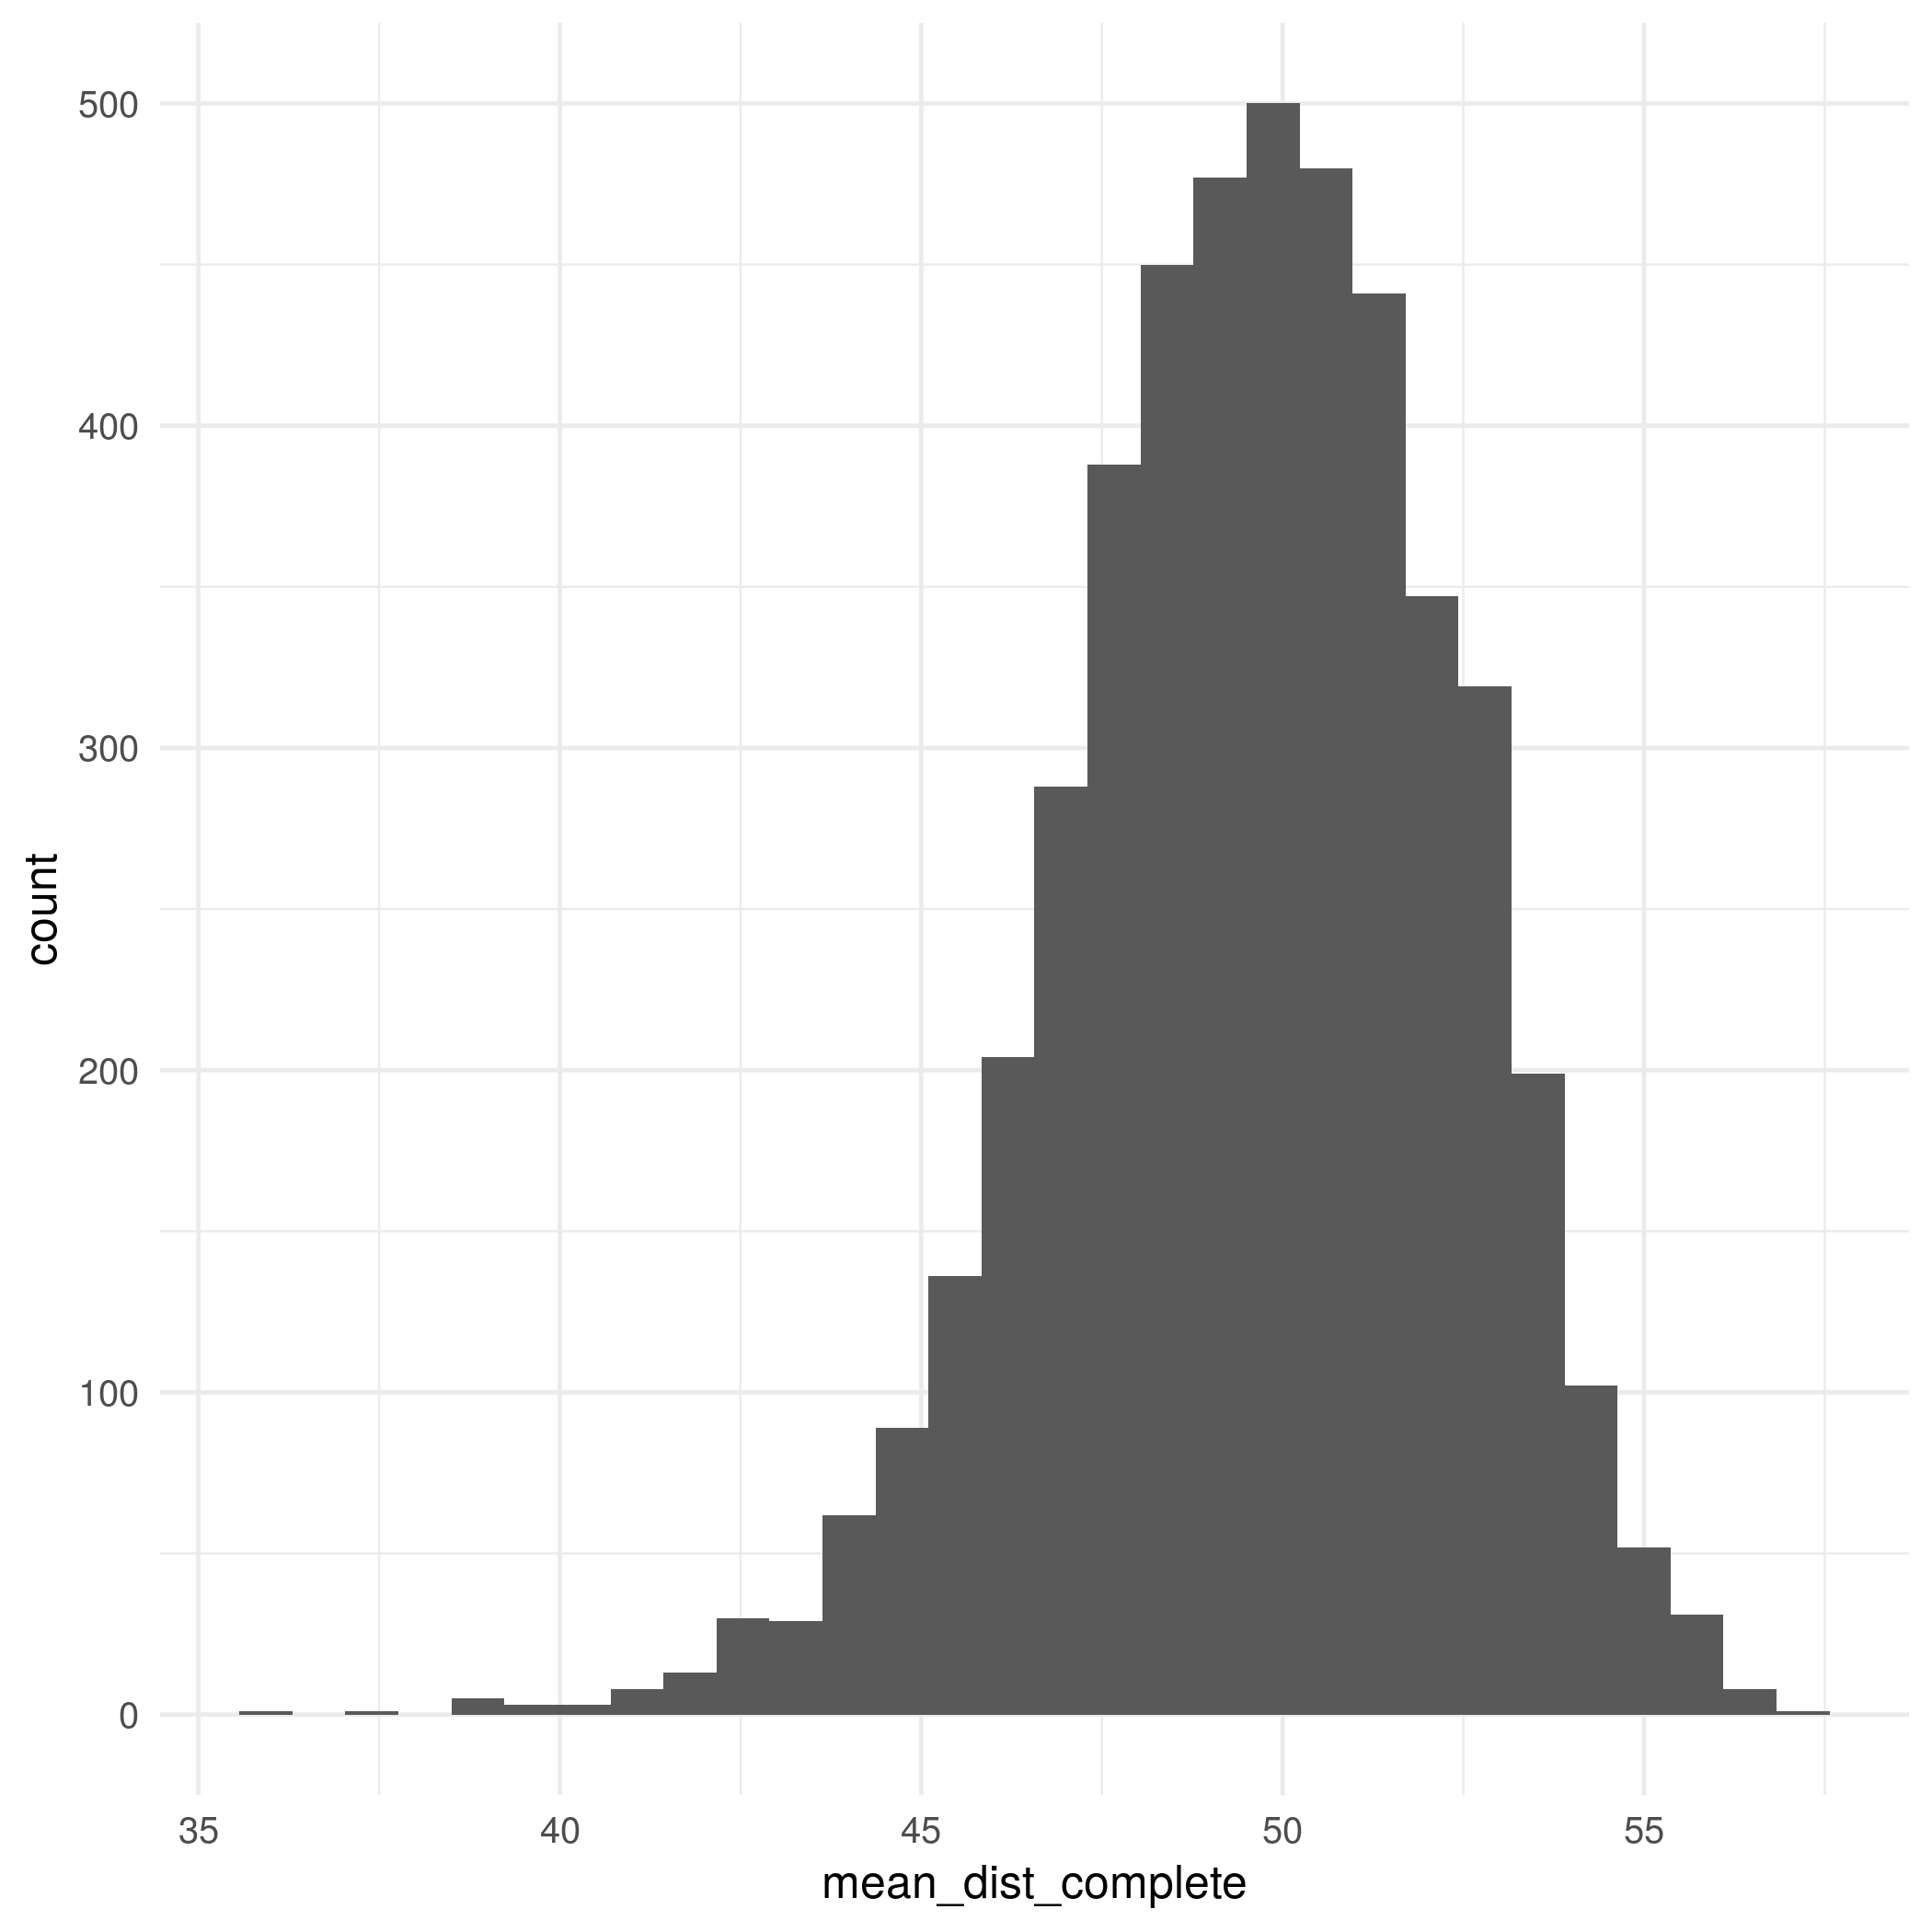
\includegraphics[width=1\linewidth]{hist_mean_dist_complete_IT000125_20190716}

\end{frame}

\begin{frame}
  \frametitle{\textbf{Pattern prediction}}

  \emph{Quantile regressions} to estimate upper and lower bounds. 
  * \textbf{Training}: 5000 small instances. 
  * \textbf{Input features}: 
    * mean flight demand per period, 
    * total remaining flight hours at start (init), 
    * variance of flight demand, 
    * demand of special missions, 
    * number of period where flight demand is cut in two. 
  * \textbf{Output features}: mean distance between maintenances.
  % TODO: add prediction results
  % TODO: add prediction example
\end{frame}

\begin{frame}
\frametitle{\textbf{Pattern filtering}}

  % TODO: add picture to explain how we filter the maintenances

  \textbf{We want to}:

  \begin{enumerate}[<+->]

  \item
    Train a statistical model to predict the mean distance between
    maintenances for any given instance.
  \item
    Use this information to limit all possible combinations of patterns to
    generate.
  \end{enumerate}

  --

  \textbf{Benefits}:

  \begin{enumerate}[<+->]

  \item
    \textbf{Performance}: a smaller model is easier to solve.
  \item
    \textbf{User feedback}: direct feedback about the solution without
    needing to solve any model.
  \item
    \textbf{More stable solutions}: Every aircraft flies an amount that is
    closest to the mean of the fleet.
  \end{enumerate}

  --

  \textbf{The better we're able to predict the optimal distance between
  maintenances for the whole fleet, the less optimality we will lose}
\end{frame}

\begin{frame}
\frametitle{\textbf{Pattern recycling}}

  % TODO: add picture to explain how we keep some

\end{frame}


\begin{frame}

\begin{block}{Experiments}

\begin{itemize}[<+->]

\item
  Number of instances: medium (1000), large (1000) and very large
  (1000).
\item
  Time limit at 3600 seconds.
\item
  We seeded instance generation for better comparison.
\item
  CPLEX running 1 thread.
\end{itemize}

--

Largest instances have 60 aircraft, 90 periods, \textasciitilde{}30
missions (4 active missions at any given time).

\begin{enumerate}[<+->]

\item
  Create forecasting model based in 5000 small instances.
\item
  Use forecasting model to predict bounds on distance between
  maintenances: \(\hat{\mu}_{t'-t}^{lb}\), \(\hat{\mu}_{t'-t}^{ub}\).
\item
  Implement the pseudo-cut:
\end{enumerate}

\begin{align}
    & m_{ip} = 0 & p_{t'} - p_t < \hat{\mu}_{t'-t}^{lb} - tol \label{eq:dist_lb} \\
    & m_{ip} = 0  &  p_{t'} - p_t > \hat{\mu}_{t'-t}^{ub} + tol \label{eq:dist_ub}
\end{align}

\begin{enumerate}[<+->]
\setcounter{enumi}{3}

\item
  Recycling.
\end{enumerate}

\end{block}

\end{frame}

\begin{frame}

\begin{block}{How good is it (performance)}

Faster solutions, more solutions.

--

.center{[}

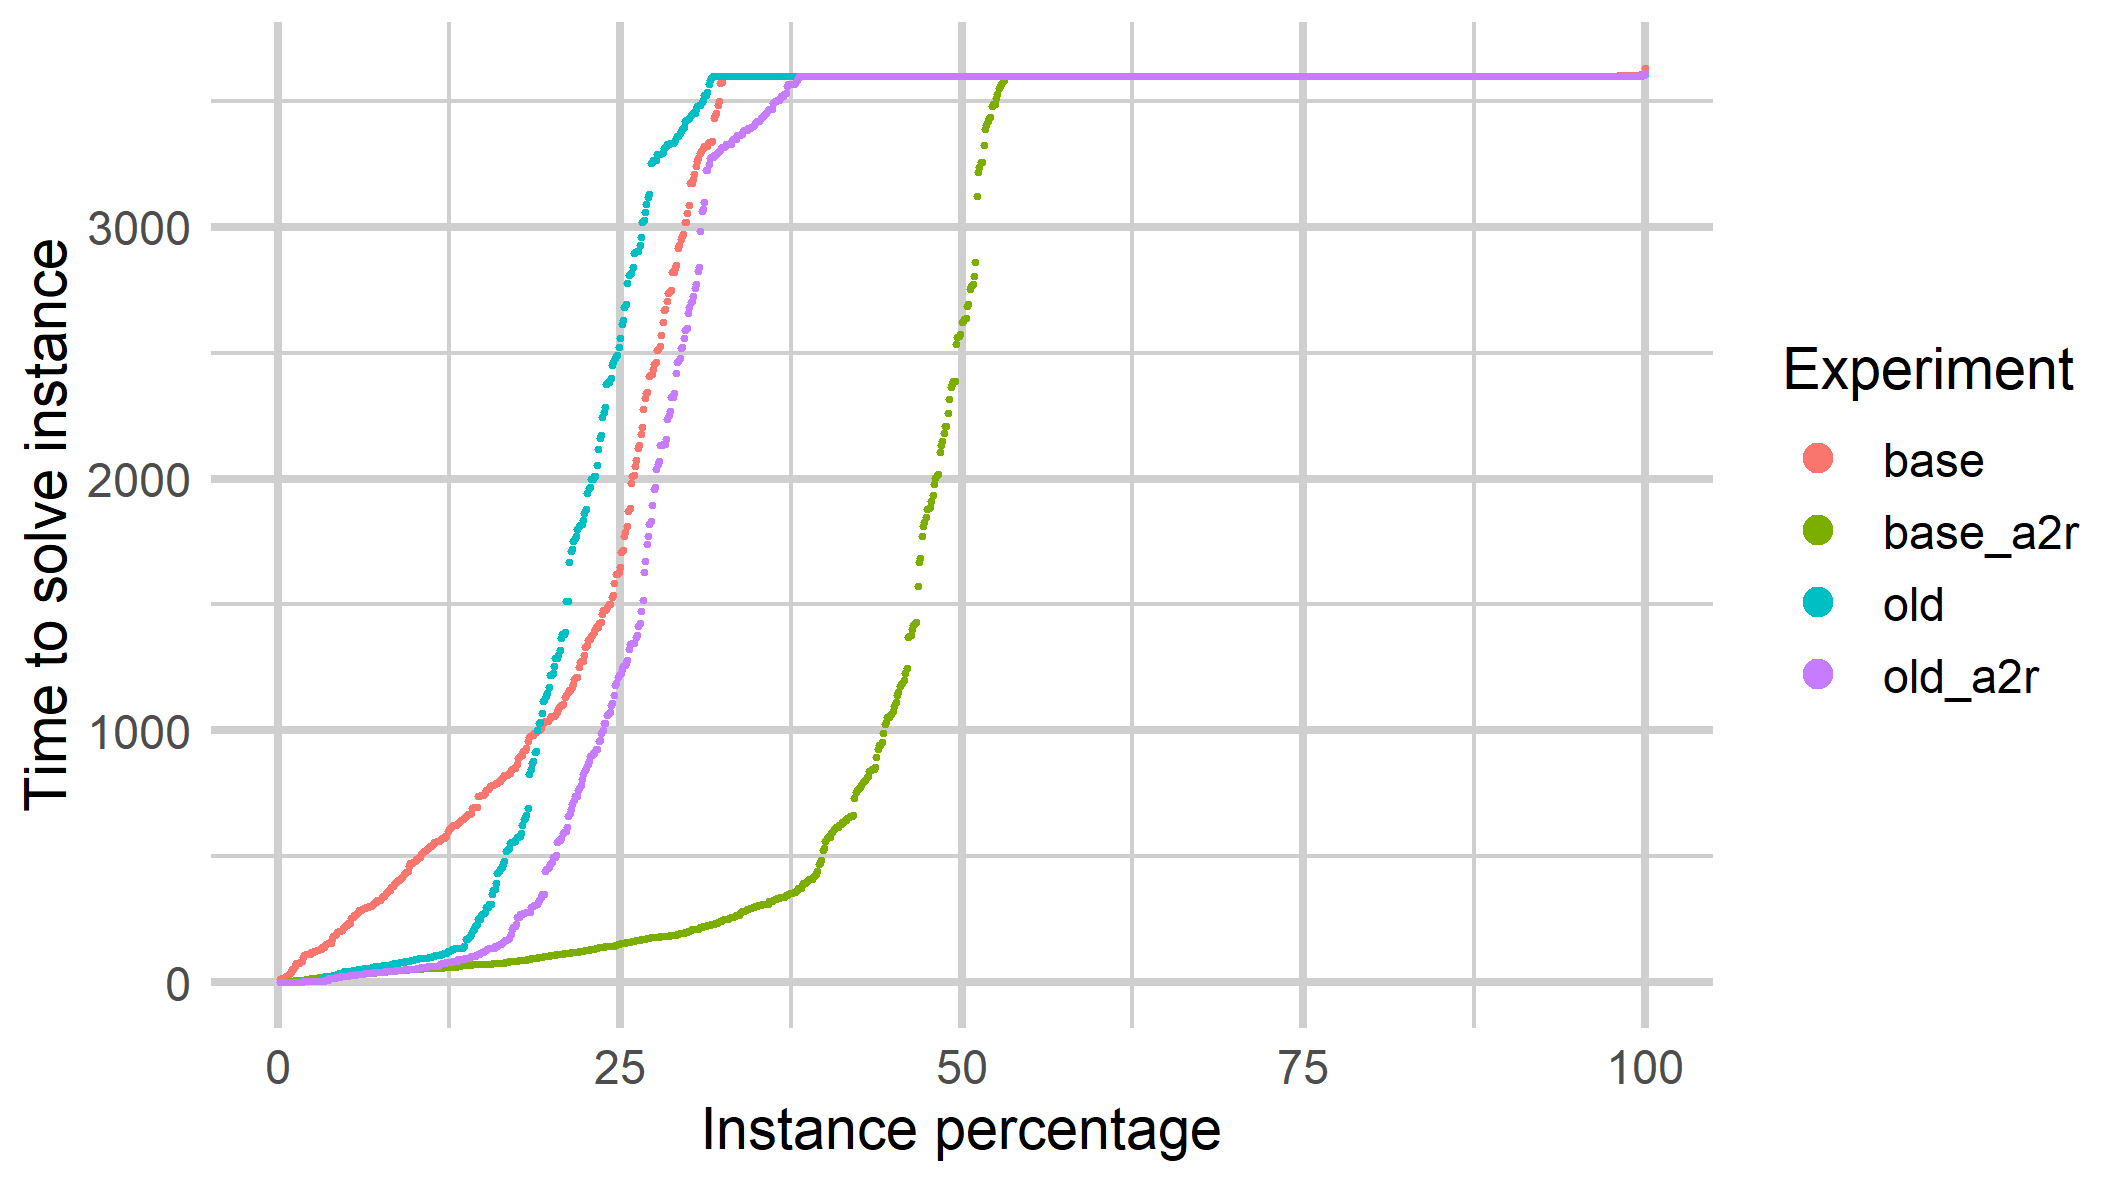
\includegraphics[width=0.8\linewidth]{time_performance_ordered_2tasks}
{]}

\end{block}

\end{frame}

\begin{frame}

\begin{block}{How good is it (optimality)}

For instances were an optimal solution was found (optimum degradation):
* 95\% of instances had less than 4\% gap with real optimal.

.center{[}

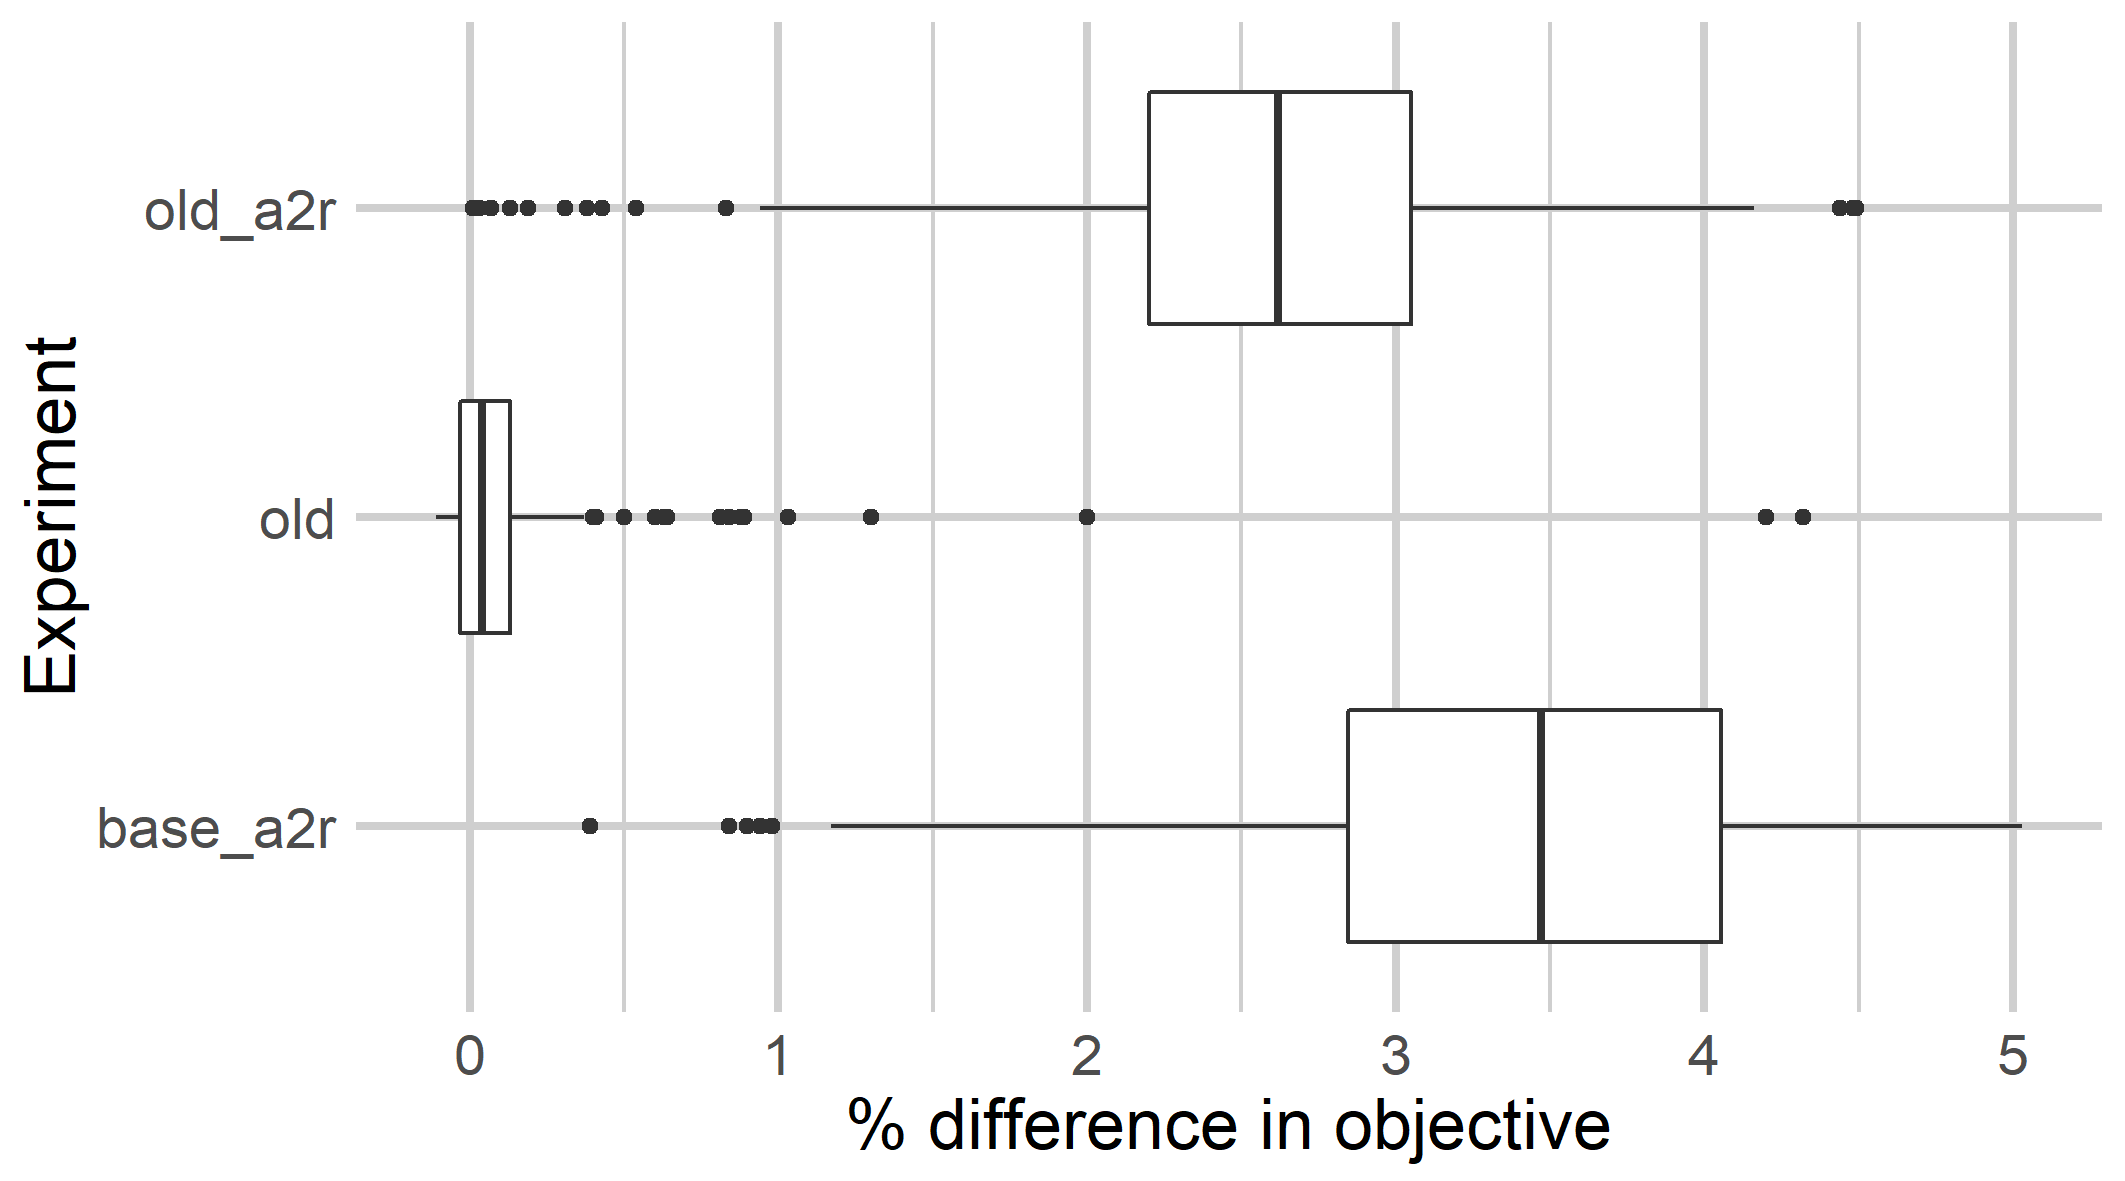
\includegraphics[width=0.8\linewidth]{quality_degradation_2tasks} {]}

\end{block}

\end{frame}

\begin{frame}{Further steps}
\protect\hypertarget{further-steps}{}

\begin{itemize}[<+->]

\item
  \textbf{Better predictions} with better features, or predicting
  several characteristics of optimal solutions.
\item
  \textbf{Predict a distribution} and sample patterns from the
  distribution instead of predicting patterns.
\item
  \textbf{Warm-start Column Generation} with a selected subset of
  potentially good patterns.
\item
  \textbf{Automatize prediction} so it can be easily integrated in other
  problems.
\end{itemize}

\end{frame}